%! \usetikzlibrary{decorations.pathreplacing,decorations.pathmorphing}
\usetikzlibrary{decorations.pathmorphing,decorations.markings}
\providecommand{\ket}[1]{\left|#1\right\rangle}
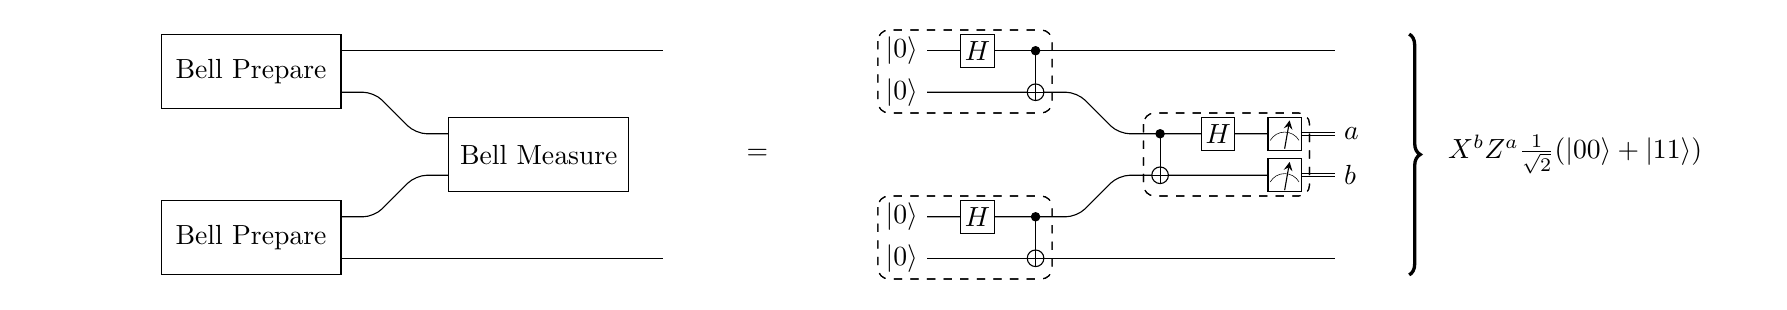
\begin{tikzpicture}[scale=1.000000,x=1pt,y=1pt]
\filldraw[color=white] (0.000000, -7.500000) rectangle (625.000000, 82.500000);
% Drawing wires
% Line 11: x W {} {} {\ket{0}} {}
\draw[color=white] (21.000000,75.000000) -- (80.500000,75.000000);
\draw[color=black] (80.500000,75.000000) -- (125.000000,75.000000);
\draw[color=black] (125.000000,75.000000) -- (132.500000,75.000000);
\draw[color=black] (132.500000,75.000000) -- (140.000000,75.000000);
\draw[color=black] (140.000000,75.000000) -- (236.500000,75.000000);
\draw[color=black] (317.500000,75.000000) -- (379.000000,75.000000);
\draw[color=black] (379.000000,75.000000) -- (386.500000,75.000000);
\draw[color=black] (386.500000,75.000000) -- (394.000000,75.000000);
\draw[color=black] (394.000000,75.000000) -- (479.500000,75.000000);
% Line 12: y W {} {} {\ket{0}} {a}
\draw[color=white] (21.000000,60.000000) -- (80.500000,60.000000);
\draw[color=black,rounded corners=4.000000pt] (80.500000,60.000000) -- (125.000000,60.000000) -- (132.500000,52.500000);
\draw[color=black,rounded corners=4.000000pt] (132.500000,52.500000) -- (140.000000,45.000000) -- (184.500000,45.000000);
\draw[color=white] (184.500000,45.000000) -- (236.500000,45.000000);
\draw[color=black,rounded corners=4.000000pt] (317.500000,60.000000) -- (379.000000,60.000000) -- (386.500000,52.500000);
\draw[color=black,rounded corners=4.000000pt] (386.500000,52.500000) -- (394.000000,45.000000) -- (454.000000,45.000000);
\draw[color=black] (454.000000,44.500000) -- (479.500000,44.500000);
\draw[color=black] (454.000000,45.500000) -- (479.500000,45.500000);
% Line 13: buf1 W
\draw[color=white] (13.500000,45.000000) -- (28.500000,45.000000);
% Line 14: buf2 W
\draw[color=white] (13.500000,30.000000) -- (28.500000,30.000000);
% Line 15: z W {} {} {\ket{0}} {b}
\draw[color=white] (21.000000,15.000000) -- (80.500000,15.000000);
\draw[color=black,rounded corners=4.000000pt] (80.500000,15.000000) -- (125.000000,15.000000) -- (132.500000,22.500000);
\draw[color=black,rounded corners=4.000000pt] (132.500000,22.500000) -- (140.000000,30.000000) -- (184.500000,30.000000);
\draw[color=white] (184.500000,30.000000) -- (236.500000,30.000000);
\draw[color=black,rounded corners=4.000000pt] (317.500000,15.000000) -- (379.000000,15.000000) -- (386.500000,22.500000);
\draw[color=black,rounded corners=4.000000pt] (386.500000,22.500000) -- (394.000000,30.000000) -- (454.000000,30.000000);
\draw[color=black] (454.000000,29.500000) -- (479.500000,29.500000);
\draw[color=black] (454.000000,30.500000) -- (479.500000,30.500000);
% Line 16: w W {} {} {\ket{0}} {}
\draw[color=white] (21.000000,0.000000) -- (80.500000,0.000000);
\draw[color=black] (80.500000,0.000000) -- (125.000000,0.000000);
\draw[color=black] (125.000000,0.000000) -- (132.500000,0.000000);
\draw[color=black] (132.500000,0.000000) -- (140.000000,0.000000);
\draw[color=black] (140.000000,0.000000) -- (236.500000,0.000000);
\draw[color=black] (317.500000,0.000000) -- (379.000000,0.000000);
\draw[color=black] (379.000000,0.000000) -- (386.500000,0.000000);
\draw[color=black] (386.500000,0.000000) -- (394.000000,0.000000);
\draw[color=black] (394.000000,0.000000) -- (479.500000,0.000000);
% Done with wires; drawing gates
% Line 18: x START x:color=white
\draw[color=white] (28.500000,75.000000) node[fill=white,left,minimum height=15.000000pt,minimum width=15.000000pt,inner sep=0pt] {\phantom{${}$}};
\draw[color=white] (28.500000,75.000000) node[left] {${}$};
% Line 19: y START y:color=white
\draw[color=white] (28.500000,60.000000) node[fill=white,left,minimum height=15.000000pt,minimum width=15.000000pt,inner sep=0pt] {\phantom{${}$}};
\draw[color=white] (28.500000,60.000000) node[left] {${}$};
% Line 20: z START z:color=white
\draw[color=white] (28.500000,15.000000) node[fill=white,left,minimum height=15.000000pt,minimum width=15.000000pt,inner sep=0pt] {\phantom{${}$}};
\draw[color=white] (28.500000,15.000000) node[left] {${}$};
% Line 21: w START w:color=white
\draw[color=white] (28.500000,0.000000) node[fill=white,left,minimum height=15.000000pt,minimum width=15.000000pt,inner sep=0pt] {\phantom{${}$}};
\draw[color=white] (28.500000,0.000000) node[left] {${}$};
% Line 22: buf1 START buf1:color=white; buf1 END
% Line 22: buf1 START buf1:color=white; buf1 END
% Line 23: buf2 START buf2:color=white; buf2 END
% Line 23: buf2 START buf2:color=white; buf2 END
% Line 26: x y G {Bell Prepare} width=65 x:color=black y:color=black
\draw (80.500000,75.000000) -- (80.500000,60.000000);
\begin{scope}
\draw[fill=white] (80.500000, 67.500000) +(-45.000000:45.961941pt and 19.091883pt) -- +(45.000000:45.961941pt and 19.091883pt) -- +(135.000000:45.961941pt and 19.091883pt) -- +(225.000000:45.961941pt and 19.091883pt) -- cycle;
\clip (80.500000, 67.500000) +(-45.000000:45.961941pt and 19.091883pt) -- +(45.000000:45.961941pt and 19.091883pt) -- +(135.000000:45.961941pt and 19.091883pt) -- +(225.000000:45.961941pt and 19.091883pt) -- cycle;
\draw (80.500000, 67.500000) node {{Bell Prepare}};
\end{scope}
% Line 27: z w G {Bell Prepare} width=65 z:color=black w:color=black
\draw (80.500000,15.000000) -- (80.500000,0.000000);
\begin{scope}
\draw[fill=white] (80.500000, 7.500000) +(-45.000000:45.961941pt and 19.091883pt) -- +(45.000000:45.961941pt and 19.091883pt) -- +(135.000000:45.961941pt and 19.091883pt) -- +(225.000000:45.961941pt and 19.091883pt) -- cycle;
\clip (80.500000, 7.500000) +(-45.000000:45.961941pt and 19.091883pt) -- +(45.000000:45.961941pt and 19.091883pt) -- +(135.000000:45.961941pt and 19.091883pt) -- +(225.000000:45.961941pt and 19.091883pt) -- cycle;
\draw (80.500000, 7.500000) node {{Bell Prepare}};
\end{scope}
% Line 29: x buf1 y z buf2 w PERMUTE
% Line 31: y z G {Bell Measure} width=65 z:color=white y:color=white
\draw (184.500000,45.000000) -- (184.500000,30.000000);
\begin{scope}
\draw[fill=white] (184.500000, 37.500000) +(-45.000000:45.961941pt and 19.091883pt) -- +(45.000000:45.961941pt and 19.091883pt) -- +(135.000000:45.961941pt and 19.091883pt) -- +(225.000000:45.961941pt and 19.091883pt) -- cycle;
\clip (184.500000, 37.500000) +(-45.000000:45.961941pt and 19.091883pt) -- +(45.000000:45.961941pt and 19.091883pt) -- +(135.000000:45.961941pt and 19.091883pt) -- +(225.000000:45.961941pt and 19.091883pt) -- cycle;
\draw (184.500000, 37.500000) node {{Bell Measure}};
\end{scope}
% Line 33: x y z w END
\draw[color=black] (229.000000,75.000000) node[fill=white,right,minimum height=15.000000pt,minimum width=15.000000pt,inner sep=0pt] {\phantom{${}$}};
\draw[color=black] (229.000000,75.000000) node[right] {${}$};
\draw[color=white] (229.000000,45.000000) node[fill=white,right,minimum height=15.000000pt,minimum width=15.000000pt,inner sep=0pt] {\phantom{${}$}};
\draw[color=white] (229.000000,45.000000) node[right] {${}$};
\draw[color=white] (229.000000,30.000000) node[fill=white,right,minimum height=15.000000pt,minimum width=15.000000pt,inner sep=0pt] {\phantom{${}$}};
\draw[color=white] (229.000000,30.000000) node[right] {${}$};
\draw[color=black] (229.000000,0.000000) node[fill=white,right,minimum height=15.000000pt,minimum width=15.000000pt,inner sep=0pt] {\phantom{${}$}};
\draw[color=black] (229.000000,0.000000) node[right] {${}$};
% Line 35: =
\draw[fill=white,color=white] (256.000000, -6.000000) rectangle (271.000000, 81.000000);
\draw (263.500000, 37.500000) node {$=$};
% Line 37: x y buf1 buf2 z w PERMUTE
% Line 39: x START x:color=black
\draw[color=black] (325.000000,75.000000) node[fill=white,left,minimum height=15.000000pt,minimum width=15.000000pt,inner sep=0pt] {\phantom{${\ket{0}}$}};
\draw[color=black] (325.000000,75.000000) node[left] {${\ket{0}}$};
% Line 40: y START y:color=black
\draw[color=black] (325.000000,60.000000) node[fill=white,left,minimum height=15.000000pt,minimum width=15.000000pt,inner sep=0pt] {\phantom{${\ket{0}}$}};
\draw[color=black] (325.000000,60.000000) node[left] {${\ket{0}}$};
% Line 41: z START z:color=black
\draw[color=black] (325.000000,15.000000) node[fill=white,left,minimum height=15.000000pt,minimum width=15.000000pt,inner sep=0pt] {\phantom{${\ket{0}}$}};
\draw[color=black] (325.000000,15.000000) node[left] {${\ket{0}}$};
% Line 42: w START w:color=black
\draw[color=black] (325.000000,0.000000) node[fill=white,left,minimum height=15.000000pt,minimum width=15.000000pt,inner sep=0pt] {\phantom{${\ket{0}}$}};
\draw[color=black] (325.000000,0.000000) node[left] {${\ket{0}}$};
% Line 44: x G $H$
\begin{scope}
\draw[fill=white] (343.000000, 75.000000) +(-45.000000:8.485281pt and 8.485281pt) -- +(45.000000:8.485281pt and 8.485281pt) -- +(135.000000:8.485281pt and 8.485281pt) -- +(225.000000:8.485281pt and 8.485281pt) -- cycle;
\clip (343.000000, 75.000000) +(-45.000000:8.485281pt and 8.485281pt) -- +(45.000000:8.485281pt and 8.485281pt) -- +(135.000000:8.485281pt and 8.485281pt) -- +(225.000000:8.485281pt and 8.485281pt) -- cycle;
\draw (343.000000, 75.000000) node {$H$};
\end{scope}
% Line 47: z G $H$
\begin{scope}
\draw[fill=white] (343.000000, 15.000000) +(-45.000000:8.485281pt and 8.485281pt) -- +(45.000000:8.485281pt and 8.485281pt) -- +(135.000000:8.485281pt and 8.485281pt) -- +(225.000000:8.485281pt and 8.485281pt) -- cycle;
\clip (343.000000, 15.000000) +(-45.000000:8.485281pt and 8.485281pt) -- +(45.000000:8.485281pt and 8.485281pt) -- +(135.000000:8.485281pt and 8.485281pt) -- +(225.000000:8.485281pt and 8.485281pt) -- cycle;
\draw (343.000000, 15.000000) node {$H$};
\end{scope}
% Line 45: x +y
\draw (364.000000,75.000000) -- (364.000000,60.000000);
\filldraw (364.000000, 75.000000) circle(1.500000pt);
\begin{scope}
\draw[fill=white] (364.000000, 60.000000) circle(3.000000pt);
\clip (364.000000, 60.000000) circle(3.000000pt);
\draw (361.000000, 60.000000) -- (367.000000, 60.000000);
\draw (364.000000, 57.000000) -- (364.000000, 63.000000);
\end{scope}
% Line 48: z +w
\draw (364.000000,15.000000) -- (364.000000,0.000000);
\filldraw (364.000000, 15.000000) circle(1.500000pt);
\begin{scope}
\draw[fill=white] (364.000000, 0.000000) circle(3.000000pt);
\clip (364.000000, 0.000000) circle(3.000000pt);
\draw (361.000000, 0.000000) -- (367.000000, 0.000000);
\draw (364.000000, -3.000000) -- (364.000000, 3.000000);
\end{scope}
% Line 50: x buf1 y z buf2 w PERMUTE
% Line 52: y +z
\draw (409.000000,45.000000) -- (409.000000,30.000000);
\filldraw (409.000000, 45.000000) circle(1.500000pt);
\begin{scope}
\draw[fill=white] (409.000000, 30.000000) circle(3.000000pt);
\clip (409.000000, 30.000000) circle(3.000000pt);
\draw (406.000000, 30.000000) -- (412.000000, 30.000000);
\draw (409.000000, 27.000000) -- (409.000000, 33.000000);
\end{scope}
% Line 53: y G $H$
\begin{scope}
\draw[fill=white] (430.000000, 45.000000) +(-45.000000:8.485281pt and 8.485281pt) -- +(45.000000:8.485281pt and 8.485281pt) -- +(135.000000:8.485281pt and 8.485281pt) -- +(225.000000:8.485281pt and 8.485281pt) -- cycle;
\clip (430.000000, 45.000000) +(-45.000000:8.485281pt and 8.485281pt) -- +(45.000000:8.485281pt and 8.485281pt) -- +(135.000000:8.485281pt and 8.485281pt) -- +(225.000000:8.485281pt and 8.485281pt) -- cycle;
\draw (430.000000, 45.000000) node {$H$};
\end{scope}
% Line 54: y M; z M
\draw[fill=white] (448.000000, 39.000000) rectangle (460.000000, 51.000000);
\draw[very thin] (454.000000, 45.600000) arc (90:150:6.000000pt);
\draw[very thin] (454.000000, 45.600000) arc (90:30:6.000000pt);
\draw[->,>=stealth] (454.000000, 39.600000) -- +(80:10.392305pt);
% Line 54: y M; z M
\draw[fill=white] (448.000000, 24.000000) rectangle (460.000000, 36.000000);
\draw[very thin] (454.000000, 30.600000) arc (90:150:6.000000pt);
\draw[very thin] (454.000000, 30.600000) arc (90:30:6.000000pt);
\draw[->,>=stealth] (454.000000, 24.600000) -- +(80:10.392305pt);
% Line 57: x y z w END
\draw[color=black] (472.000000,75.000000) node[fill=white,right,minimum height=15.000000pt,minimum width=15.000000pt,inner sep=0pt] {\phantom{${}$}};
\draw[color=black] (472.000000,75.000000) node[right] {${}$};
\draw[color=black] (472.000000,45.000000) node[fill=white,right,minimum height=15.000000pt,minimum width=15.000000pt,inner sep=0pt] {\phantom{${a}$}};
\draw[color=black] (472.000000,45.000000) node[right] {${a}$};
\draw[color=black] (472.000000,30.000000) node[fill=white,right,minimum height=15.000000pt,minimum width=15.000000pt,inner sep=0pt] {\phantom{${b}$}};
\draw[color=black] (472.000000,30.000000) node[right] {${b}$};
\draw[color=black] (472.000000,0.000000) node[fill=white,right,minimum height=15.000000pt,minimum width=15.000000pt,inner sep=0pt] {\phantom{${}$}};
\draw[color=black] (472.000000,0.000000) node[right] {${}$};
% Line 59: x w >= $X^{b}Z^{a}\frac{1}{\sqrt{2}}(\ket{00}+\ket{11})$ width=120
\draw[fill=white,color=white] (499.000000, -6.000000) rectangle (619.000000, 81.000000);
\draw (559.000000, 37.500000) node {$X^{b}Z^{a}\frac{1}{\sqrt{2}}(\ket{00}+\ket{11})$};
\draw[decorate,decoration={brace,mirror,amplitude = 4.000000pt},very thick] (499.000000,-6.000000) -- (499.000000,81.000000);
% Done with gates; drawing ending labels
% Done with ending labels; drawing cut lines and comments
% Line 63: x y @ 7 9 color=black style=dashed,rounded_corners=4pt
\draw[draw opacity=1.000000,fill opacity=0.200000,color=black,dashed,rounded corners=4pt] (307.000000,82.500000) rectangle (370.000000,52.500000);
\draw[draw opacity=1.000000,fill opacity=0.200000,color=black,dashed,rounded corners=4pt] (307.000000,82.500000) rectangle (370.000000,52.500000);
% Line 64: z w @ 7 9 color=black style=dashed,rounded_corners=4pt
\draw[draw opacity=1.000000,fill opacity=0.200000,color=black,dashed,rounded corners=4pt] (307.000000,22.500000) rectangle (370.000000,-7.500000);
\draw[draw opacity=1.000000,fill opacity=0.200000,color=black,dashed,rounded corners=4pt] (307.000000,22.500000) rectangle (370.000000,-7.500000);
% Line 66: y z @ 11 13 color=black style=dashed,rounded_corners=4pt
\draw[draw opacity=1.000000,fill opacity=0.200000,color=black,dashed,rounded corners=4pt] (403.000000,52.500000) rectangle (463.000000,22.500000);
\draw[draw opacity=1.000000,fill opacity=0.200000,color=black,dashed,rounded corners=4pt] (403.000000,52.500000) rectangle (463.000000,22.500000);
% Done with comments
\end{tikzpicture}
